%{{第六十二回}}{第六十二回}}

\chapter{憨湘云醉眠芍药裀 呆香菱情解石榴裙}

{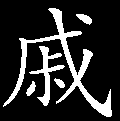
\includegraphics[width=3mm]{../Images/00005}众姊妹一番赠}贶{,诸僧尼一番祷祝,确是宝玉生辰。园中行礼,不亢不卑,席上设筵,不丰不啬,确是宝玉分地。}

{探春围棋理事,气象严厉;香菱斗草善谑,姿态俊逸。湘云喜饮酒,何等疏爽;黛玉怕吃茶,何等妩媚。晴雯刺芳官,语极尖利;袭人给裙子,意极醇良。字字曲到。}

话说平儿出来吩咐林之孝家的道:``大事化为小事,小事化为没事,方是兴旺之家。若得不了一点子小事,便扬铃打鼓的乱折腾起来,不成道理。如今将他母女带回,照旧去当差。将秦显家的仍旧退回。再不必提此事。只是每日小心巡察要紧。''说毕,起身走了。柳家的母女忙向上磕头,林家的带回园中,回了李纨探春,二人皆说:``知道了,能可无事,很好。''

司棋等人空兴头了一阵。那秦显家的好容易等了这个空子钻了来,只兴头上半天。在厨房内正乱着接收家伙、米粮、煤炭等物,又查出许多亏空来,说:``粳米短了两石,常用米又多支了一个月的,炭也欠着额数。''一面又打点送林之孝家的礼,悄悄的备了一篓炭,五百斤木柴,一担粳米,在外边就遣了子侄送入林家去了;又打点送账房的礼;又预备几样菜蔬请几位同事的人,说:``我来了,全仗列位扶持。自今以后都是一家人了。我有照顾不到的,好歹大家照顾些。''

正乱着,忽有人来说与他:``看过这早饭就出去罢。柳嫂儿原无事,如今还交与他管了。''秦显家的听了,轰去魂魄,垂头丧气,登时掩旗息鼓,卷包而出。送人之物白丢了许多,自己倒要折变了赔补亏空。连司棋都气了个倒仰,无计挽回,只得罢了。

赵姨娘正因彩云私赠了许多东西,被玉钏儿吵出,生恐查诘出来,每日捏一把汗打听信儿。忽见彩云来告诉说:``都是宝玉应了,从此无事。''赵姨娘方把心放下来。谁知贾环听如此说,便起了疑心,将彩云凡私赠之物都拿了出来,照着彩云的脸摔了去,说:``这两面三刀的东西!我不稀罕。你不和宝玉好,他如何肯替你应。你既有担当给了我,原该不与一个人知道。如今你既然告诉他,如今我再要这个,也没趣儿。''彩云见如此,急的发身赌誓,至于哭了,百般解说,贾环执意不信,说:``不看你素日之情,去告诉二嫂子,就说你偷来给我,我不敢要。你细想去。''说毕,摔手出去了。急的赵姨娘骂:``没造化的种子,蛆心孽障。''气的彩云哭个泪干肠断。赵姨娘百般的安慰他:``好孩子,他辜负了你的心,我看的真。让我收起来,过两日他自然回转过来了。''说着,便要收东西。彩云赌气一顿包起来,乘人不见时,来至园中,都撇在河内,顺水沉的沉漂的漂了。自己气的夜间在被内暗哭。

当下又值宝玉生日已到,原来宝琴也是这日,二人相同。因王夫人不在家,也不曾像往年闹热。只有张道士送了四样礼,换的寄名符儿;还有几处僧尼庙的和尚姑子送了供尖儿,并寿星纸马疏头,并本命星官值年太岁周年换的锁儿。家中常走的女先儿来上寿。王子腾那边,仍是一套衣服,一双鞋袜,一百寿桃,一百束上用银丝挂面。薛姨娘处减一等。其馀家中人,尤氏仍是一双鞋袜;凤姐儿是一个宫制四面和合荷包,里面装一个金寿星,一件波斯国所制玩器。各庙中遣人去放堂舍钱。又另有宝琴之礼,不能备述。姐妹中皆随便,或有一扇的,或有一字的,或有一画的,或有一诗的,聊复应景而已。

这日宝玉清晨起来,梳洗已毕,冠带出来。至前厅院中,已有李贵等四五个人在那里设下天地香烛,宝玉炷了香。行毕礼,奠茶焚纸后,便至宁府中宗祠祖先堂两处行毕礼,出至月台上,又朝上遥拜过贾母、贾政、王夫人等。一顺到尤氏上房,行过礼,坐了一回,方回荣府。先至薛姨妈处,薛姨妈再三拉着,然后又遇见薛蝌,让一回,方进园来。晴雯麝月二人跟随,小丫头夹着毡子,从李氏起,一一挨着所长的房中到过。复出二门,至李、赵、张、王四个奶妈家让了一回,方进来。虽众人要行礼,也不曾受。回至房中,袭人等只都来说一声就是了。王夫人有言,不令年轻人受礼,恐折了福寿,故皆不磕头。

歇一时,贾环贾兰等来了,袭人连忙拉住,坐了一坐,便去了。宝玉笑说走乏了,便歪在床上。方吃了半盏茶,只听外面咭咭呱呱,一群丫头笑进来,原来是翠墨、小螺、翠缕、入画,邢岫烟的丫头篆儿,并奶子抱巧姐儿,彩鸾、绣鸾八九个人,都抱着红毡笑着走来,说:``拜寿的挤破了门了,快拿面来我们吃。''刚进来时,探春、湘云、宝琴、岫烟、惜春也都来了。宝玉忙迎出来,笑说:``不敢起动,快预备好茶。''进入房中,不免推让一回,大家归坐。袭人等捧过茶来,才吃了一口,平儿也打扮的花枝招展的来了。宝玉忙迎出来,笑说:``我方才到凤姐姐门上,回了进去,不能见,我又打发人进去让姐姐的。''平儿笑道:``我正打发你姐姐梳头,不得出来回你。后来听见又说让我,我那里禁当的起,所以特赶来磕头。''宝玉笑道:``我也禁当不起。''袭人早在外间安了坐,让他坐。平儿便福下去,宝玉作揖不迭。平儿便跪下去,宝玉也忙还跪下,袭人连忙搀起来。又下了福,宝玉又还了一揖。袭人笑推宝玉:``你再作揖。''宝玉道:``已经完了,怎么又作揖?''袭人笑道:``这是他来给你拜寿。今儿也是他的生日,你也该给他拜寿。''宝玉听了,喜的忙作下揖去,说:``原来今儿也是姐姐的芳诞。''平儿还万福不迭。湘云拉宝琴岫烟说:``你们四个人对拜寿,直拜一天才是。''探春忙问:``原来邢妹妹也是今儿?我怎么就忘了。''忙命丫头:``去告诉二奶奶,赶着补了一分礼,与琴姑娘的一样,送到二姑娘屋里去。''丫头答应着去了。岫烟见湘云直口说出来,少不得要到各房去让让。

探春笑道:``倒有些意思,一年十二个月,月月有几个生日。人多了,便这等巧,也有三个一日、两个一日的。大年初一日也不白过,大姐姐占了去。怨不得他福大,生日比别人就占先。又是太祖太爷的生日。过了灯节,就是老太太和宝姐姐,他们娘儿两个遇的巧。三月初一日是太太,初九日是琏二哥哥。二月没人。''袭人道:``二月十二是林姑娘,怎么没人?就只不是咱家的人。''探春笑道:``我这个记性是怎么了!''宝玉笑指袭人道:``他和林妹妹是一日,所以他记的。''探春笑道:``原来你两个倒是一日。每年连头也不给我们磕一个。平儿的生日我们也不知道,这也是才知道。''平儿笑道:``我们是那牌儿名上的人,生日也没拜寿的福,又没受礼职份,可吵闹什么,可不悄悄的过去。今儿他又偏吵出来了,等姑娘们回房,我再行礼去罢。''探春笑道:``也不敢惊动。只是今儿倒要替你过个生日,我心才过得去。''宝玉湘云等一齐都说:``很是。''探春便吩咐了丫头:``去告诉他奶奶,就说我们大家说了,今儿一日不放平儿出去,我们也大家凑了分子过生日呢。''丫头笑着去了,半日,回来说:``二奶奶说了,多谢姑娘们给他脸。不知过生日给他些什么吃,只别忘了二奶奶,就不来絮聒他了。''众人都笑了。

探春因说道:``可巧今儿里头厨房不预备饭,一应下面弄菜都是外头收拾。咱们就凑了钱叫柳家的来揽了去,只在咱们里头收拾倒好。''众人都说是极。探春一面遣人去问李纨、宝钗、黛玉,一面遣人去传柳家的进来,吩咐他内厨房中快收拾两桌酒席。柳家的不知何意,因说外厨房都预备了。探春笑道:``你原来不知道,今儿是平姑娘的华诞。外头预备的是上头的,这如今我们私下又凑了分子,单为平姑娘预备两桌请他。你只管拣新巧的菜蔬预备了来,开了账和我那里领钱。''柳家的笑道:``原来今日也是平姑娘的千秋,我竟不知道。''说着,便向平儿磕下头去,慌的平儿拉起他来。柳家的忙去预备酒席。

这里探春又邀了宝玉,同到厅上去吃面,等到李纨宝钗一齐来全,又遣人去请薛姨妈与黛玉。因天气和暖,黛玉之疾渐愈,故也来了。花团锦簇,挤了一厅的人。

谁知薛蝌又送了巾扇香帛四色寿礼与宝玉,宝玉于是过去陪他吃面。两家皆治了寿酒,互相酬送,彼此同领。至午间,宝玉又陪薛蝌吃了两杯酒。宝钗带了宝琴过来与薛蝌行礼,把盏毕,宝钗因嘱薛蝌:``家里的酒也不用送过那边去,这虚套竟可收了。你只请伙计们吃罢。我们和宝兄弟进去还要待人去呢,也不能陪你了。''薛蝌忙说:``姐姐兄弟只管请,只怕伙计们也就好来了。''宝玉忙又告过罪,方同他姊妹回来。

一进角门,宝钗便命婆子将门锁上,把钥匙要了自己拿着。宝玉忙说:``这一道门何必关,又没多的人走。况且姨娘、姐姐、妹妹都在里头,倘或家去取什么,岂不费事。''宝钗笑道:``小心没过逾的。你瞧你们那边,这几日七事八事,竟没有我们这边的人,可知是这门关的有功效了。若是开着,保不住那起人图顺脚,超近路从这里走,拦谁的是?不如锁了,连妈和我也禁着些,大家别走。纵有了事,就赖不着这边的人了。''宝玉笑道:``原来姐姐也知道我们那边近日丢了东西?''宝钗笑道:``你只知道玫瑰露和茯苓霜两件,乃因人而及物。若非因人,你连这两件还不知道呢。殊不知还有几件比这两件大的呢。若以后叨登不出来,是大家的造化;若叨登出来,不知里头连累多少人呢。你也是不管事的人,我才告诉你。平儿是个明白人,我前儿也告诉了他,皆因他奶奶不在外头,所以使他明白了。若不出来,大家乐得丢开手。若犯出来,他心里已有稿子,自有头绪,就冤屈不着平人了。你只听我说,以后留神小心就是了,这话也不可对第二个人讲。''

说着,来到沁芳亭边,只见袭人、香菱、待书、素云、晴雯、麝月、芳官、蕊官、藕官等十来个人都在那里看鱼作耍。见他们来了,都说:``芍药栏里预备下了,快去上席罢。''宝钗等遂携了他们同到了芍药栏中红香圃三间小敞厅内。连尤氏已请过来了,诸人都在那里,只没平儿。

原来平儿出去,有赖、林诸家送了礼来,连三接四,上中下三等家人来拜寿送礼的不少,平儿忙着打发赏钱道谢,一面又色色的回明凤姐儿,不过留下几样,也有不收的,也有收下即刻赏与人的。忙了一回,又直待凤姐儿吃过面,方换了衣裳往园里来。

刚进了园,就有几个丫鬟来找他,一同到了红香圃中。只见筵开玳瑁,褥设芙蓉。众人都笑:``寿星全了。''上面四座定要让他四个人坐,四人皆不肯。薛姨妈说:``我老天拔地,又不合你们的群儿,我倒觉拘的慌,不如我到厅上随便躺躺去倒好。我又吃不下什么去,又不大吃酒,这里让他们倒便宜。''尤氏等执意不从。宝钗道:``这也罢了,倒是让妈在厅上歪着自如些,有爱吃的送些过去,倒自在了。且前头没人在那里,又可照看了。''探春等笑道:``既这样,恭敬不如从命。''因大家送了他到议事厅上,眼看着命丫头们铺了一个锦褥并靠背引枕之类,又嘱咐:``好生给姨妈捶腿,要茶要水别推三扯四的。回来送了东西来,姨妈吃了就赏你们吃。只别离了这里出去。''小丫头们都答应了。

探春等方回来。终久让宝琴、岫烟二人在上,平儿面西坐,宝玉面东坐。探春又接了鸳鸯来,二人并肩对面相陪。西边一桌,宝钗、黛玉、湘云、迎春、惜春,一面又拉了香菱、玉钏儿二人打横。三桌上,尤氏、李纨,又拉了袭人、彩云陪坐。四桌上便是紫鹃、莺儿、晴雯、小螺、司棋等人围坐。当下探春等还要把盏,宝琴等四人都说:``这一闹,一日都坐不成了。''方才罢了。两个女先儿要弹词上寿,众人都说:``我们没人要听那些野话,你厅上去说给姨太太解闷儿去罢。''一面又将各色吃食拣了,命人送与薛姨妈去。

宝玉便说:``雅坐无趣,须要行令才好。''众人有的说行这个令好,那个又说行那个令好。黛玉道:``依我说,拿了笔砚将各色全都写了,拈成阄儿,咱们抓出那个来,就是那个。''众人都道妙。即拿了一副笔砚花笺。香菱近日学了诗,又天天学写字,见了笔砚便图不得,连忙起座说:``我写。''大家想了一回,共得了十来个,念着,香菱一一的写了,搓成阄儿,掷在一个瓶中间。探春便命平儿拣,平儿向内搅了一搅,用箸拈了一个出来,打开看,上写着``射覆''二字。宝钗笑道:``把个酒令的祖宗拈出来。`射覆'从古有的,如今失了传,这是后人纂的,比一切的令都难。这里头倒有一半是不会的,不如毁了,另拈一个雅俗共赏的。''探春笑道:``既拈了出来,如何又毁。如今再拈一个,若是雅俗共赏的,便叫他们行去。咱们行这个。''说着又着袭人拈了一个,却是``拇战''。史湘云笑着说:``这个简断爽利,合了我的脾气。我不行这个`射覆',没的垂头丧气闷人,我只划拳去了。''探春道:``惟有他乱令,宝姐姐快罚他一钟。''宝钗不容分说,便灌湘云一杯。

探春道:``我吃一杯,我是令官,也不用宣,只听我分派。''命取了令骰令盆来,``从琴妹掷起,挨下掷去,对了点的二人射覆。''宝琴一掷,是个三,岫烟宝玉等皆掷的不对,直到香菱方掷了个三。宝琴笑道:``只好室内生春,若说到外头去,可太没头绪了。''探春道:``自然。三次不中者罚一杯。你覆,他射。''宝琴想了一想,说了个``老''字。香菱原生于这令,一时想不到,满室满席都不见有与``老''字相连的成语。湘云先听了,便也乱看,忽见门斗上贴着``红香圃''三个字,便知宝琴覆的是``吾不如老圃''的``圃''字。见香菱射不着,众人击鼓又催,便悄悄的拉香菱,教他说``药''字。黛玉偏看见了,说``快罚他,又在那里私相传递呢。''哄的众人都知道了,忙又罚了一杯,恨的湘云拿筷子敲黛玉的手。于是罚了香菱一杯。下则宝钗和探春对了点子。探春便覆了一个``人''字。宝钗笑道:``这个`人'字泛的很。''探春笑道:``添一字,两覆一射也不泛了。''说着,便又说了一个``窗''字。宝钗一想,因见席上有鸡,便射着他是用``鸡窗''``鸡人''二典了,因射了一个``埘''字。探春知他射着,用了``鸡栖于埘''的典,二人一笑,各饮一口门杯。

湘云等不得,早和宝玉``三''``五''乱叫,划起拳来。那边尤氏和鸳鸯隔着席也``七''``八''乱叫划起来。平儿袭人也作了一对划拳,叮叮当当只听得腕上的镯子响。一时湘云赢了宝玉,鸳鸯赢了尤氏\href{../Text/part0066_split_000.html\#lnkback_1_a}{\textsuperscript{①}},袭人赢了平儿,三个人限酒底酒面,湘云便说:``酒面要一句古文,一句旧诗,一句骨牌名,一句曲牌名,还要一句时宪书上的话,共总凑成一句话。酒底要关人事的果菜名。''众人听了,都笑说:``惟有他的令也比人唠叨,倒也有意思。''便催宝玉快说。宝玉笑道:``谁说过这个,也等想一想儿。''黛玉便道:``你多喝一钟,我替你说。''宝玉真个喝了酒,听黛玉说道:

落霞与孤鹜齐飞,风急江天过雁哀,却是一只折足雁,叫的人九回肠,这是鸿雁来宾。

说的大家笑了,说:``这一串子倒有些意思。''黛玉又拈了一个榛穰,说酒底道:

榛子非关隔院砧,何来万户捣衣声。

令完,鸳鸯袭人等皆说的是一句俗语,都带一个``寿''字的,不能多赘。

大家轮流乱划了一阵,这上面湘云又和宝琴对了手,李纨和岫烟对了点子。李纨便覆了一个``瓢''字,岫烟便射了一个``绿''字,二人会意,各饮一口。湘云的拳却输了,请酒面酒底。宝琴笑道:``请君入瓮。''大家笑起来,说:``这个典用的当。''湘云便说道:

奔腾而砰湃,江间波浪兼天涌,须要铁锁缆孤舟,既遇着一江风,不宜出行。

说的众人都笑了,说:``好个诌断了肠子的。怪道他出这个令,故意惹人笑。''又听他说酒底。湘云吃了酒,拣了一块鸭肉呷口,忽见碗内有半个鸭头,遂拣了出来吃脑子。众人催他:``别只顾吃,到底快说了。''湘云便用箸子举着说道:

这鸭头不是那丫头,头上那讨桂花油。

众人越发笑起来,引的晴雯、小螺、莺儿等一干人都走过来说:``云姑娘会开心儿,拿着我们取笑儿,快罚一杯才罢。怎见得我们就该擦桂花油的?倒得每人给一瓶子桂花油擦擦。''黛玉笑道:``他倒有心给你们一瓶子油,又怕挂误着打盗窃的官司。''众人不理论,宝玉却明白,忙低了头。彩云有心病,不觉的红了脸。宝钗忙暗暗的瞅了黛玉一眼。黛玉自悔失言,原是趣宝玉的,就忘了趣着彩云。自悔不及,忙一顿行令划拳岔开了。

底下宝玉可巧和宝钗对了点子。宝钗覆了一个``宝''字,宝玉想了一想,便知是宝钗作戏指自己所佩通灵玉而言,便笑道:``姐姐拿我作雅谑,我却射着了。说出来姐姐别恼,就是姐姐的讳`钗'字就是了。''众人道:``怎么解?''宝玉道:``他说`宝',底下自然是`玉'了。我射`钗'字,旧诗曾有`敲断玉钗红烛冷',岂不射着了。''湘云说道:``这用时事却使不得,两个人都该罚。''香菱忙道:``不止时事,这也有出处。''湘云道:```宝玉'二字并无出处,不过是春联上或有之,诗书纪载并无,算不得。''香菱道:``前日我读岑嘉州五言律,现有一句说`此乡多宝玉',怎么你倒忘了?后来又读李义山七言绝句,又有一句`宝钗无日不生尘',我还笑说他两个名字都原来在唐诗上呢。''众人笑说:``这可问住了,快罚一杯。''湘云无语,只得饮了。大家又该对点的对点,划拳的划拳。这些人因贾母王夫人不在家,没了管束,便任意取乐,呼三喝四,喊七叫八。满厅中红飞翠舞,玉动珠摇,真是十分热闹。顽了一回,大家方起席散了一散,倏然不见了湘云,只当他外头自便就来,谁知越等越没了影响,使人各处去找,那里找得着。

接着林之孝家的同着几个老婆子来,生恐有正事呼唤,二者恐丫鬟们年青,乘王夫人不在家不服探春等约束,姿意痛饮,失了体统,故来请问有事无事。探春见他们来了,便知其意,忙笑道:``你们又不放心,来查我们来了。我们没有多吃酒,不过是大家顽笑,将酒作个引子,妈妈们别耽心。''李纨尤氏都也笑说:``你们歇着去罢,我们也不敢叫他们多吃了。''林之孝家的等人笑说:``我们知道,连老太太叫姑娘吃酒姑娘们还不肯吃,
何况太太们不在家,自然顽罢了。我们怕有事,来打听打听。二则天长了,姑娘们顽一回子还该点补些小食儿。素日又不大吃杂东西,如今吃一两杯酒,若不多吃些东西,怕受伤。''探春笑道:``妈妈们说的是,我们也正要吃呢。''因回头命取点心来。两旁丫鬟们答应了,忙去传点心。探春又笑让:``你们歇着去罢,或是姨妈那里说话儿去。我们即刻打发人送酒你们吃去。''林之孝家的等人笑回:``不敢领了。''又站了一回,方退了出来。平儿摸着脸笑道:``我的脸都热了,也不好意思见他们。依我说竟收了罢,别惹他们再来,倒没意思了。''探春笑道:``不相干,横竖咱们不认真喝酒就罢了。''

正说着,只见一个小丫头笑嘻嘻的走来:``姑娘们快瞧云姑娘去,吃醉了图凉快,在山子后头一块青板石凳上睡着了。''众人听说,都笑道:``快别吵嚷。''说着,都走来看时,果见湘云卧于山石僻处一个石凳子上,业经香梦沉酣。四面芍药花飞了一身,满头、脸、衣襟上皆是红香散乱,手中的扇子在地下,也半被落花埋了,一群蜂蝶闹穰穰的围着他,又用鲛帕包了一包芍药花瓣枕着。众人看了,又是爱,又是笑,忙上来推唤挽扶。湘云口内犹作睡语说酒令,唧唧嘟嘟说:

泉香而酒冽,玉盏盛来琥珀光,直饮到梅梢月上,醉扶归,却为宜会亲友。

众人笑推他,说道:``快醒醒儿吃饭去,这潮凳上还睡出病来呢。''湘云慢启秋波,见了众人,低头看了一看自己,方知是醉了。原是来纳凉避静的,不觉的因多罚了两杯酒,娇嫋不胜,便睡着了,心中反觉自愧。连忙起身扎挣着同人来至红香圃中,用过水,又吃了两盏酽茶。探春忙命将醒酒石拿来给他衔在口内,一时又命他喝了一些酸汤,方才觉得好了些。

当下又选了几样果菜与凤姐送去,凤姐儿也送了几样来。宝钗等吃过点心,大家也有坐的,也有立的,也有在外观花的,也有扶栏观鱼的,各自取便说笑不一。探春便和宝琴下棋,宝钗岫烟观局。林黛玉和宝玉在一簇花下唧唧哝哝不知说些什么。只见林之孝家的和一群女人带了一个媳妇进来。那媳妇愁眉苦脸,也不敢进厅,只到了阶下,便朝上跪下了,碰头有声。探春因一块棋受了敌,算来算去总得了两个眼,便折了官着,两眼只瞅着棋枰,一只手却伸在盒内,只管抓弄棋子作想,林之孝家的站了半天,因回头要茶时才看见,问:``什么事?''林之孝家的便指那媳妇说:``这是四姑娘屋里的小丫头彩儿的娘,现是园内伺候的人。嘴很不好,才是我听见了问着他,他说的话也不敢回姑娘,竟要撵出去才是。''探春道:``怎么不回大奶奶?''林之孝家的道:``方才大奶奶都往厅上姨太太处去了,顶头看见,我已回明白了,叫回姑娘来。''探春道:``怎么不回二奶奶?''平儿道:``不回去也罢,我回去说一声就是了。''探春点点头,道:``既这么着,就撵出他去,等太太来了,再回定夺。''说毕仍又下棋。这林之孝家的带了那人去不提。

黛玉和宝玉二人站在花下,遥遥知意。黛玉便说道:``你家三丫头倒是个乖人。虽然叫他管些事,倒也一步儿不肯多走。差不多的人就早作起威福来了。''宝玉道:``你不知道呢。你病着时,他干了好几件事。这园子也分了人管,如今多掐一草也不能了。又蠲了几件事,单拿我和凤姐姐作筏子禁别人。最是心里有算计的人,岂只乖而已。''黛玉道:``要这样才好,咱们家里也太花费了。我虽不管事,心里每常闲了,替你们一算计,出的多进的少,如今若不省俭,必致后手不接。''宝玉笑道:``凭他怎么后手不接,也短不了咱们两个人的。''黛玉听了,转身就往厅上寻宝钗说笑去了。

宝玉正欲走时,只见袭人走来,手内捧着一个小连环洋漆茶盘,里面可式放着两钟新茶,因问:``他往那去了?我见你两个半日没吃茶,巴巴的倒了两钟来,他又走了。''宝玉道:``那不是他,你给他送去。''说着自拿了一钟。袭人便送了那钟去,偏和宝钗在一处,只得一钟茶,便说:``那位渴了那位先接了,我再倒去。''宝钗笑道:``我却不渴,只要一口漱一漱就够了。''说着先拿起来喝了一口,剩下半杯递在黛玉手内。袭人笑说:``我再倒去。''黛玉笑道:``你知道我这病,大夫不许我多吃茶,这半钟尽够了,难为你想的到。''说毕,饮干,将杯放下。袭人又来接宝玉的。宝玉因问:``这半日没见芳官,他在那里呢?''袭人四顾一瞧说:``才在这里几个人斗草的,这会子不见了。''

宝玉听说,便忙回至房中,果见芳官面向里睡在床上。宝玉推他说道:``快别睡觉,咱们外头顽去,一回儿好吃饭的。''芳官道:``你们吃酒不理我,教我闷了半日,可不来睡觉罢了。''宝玉拉了他起来,笑道:``咱们晚上家里再吃,回来我叫袭人姐姐带了你桌上吃饭,何如?''芳官道:``藕官蕊官都不上去,单我在那里也不好。我也不惯吃那个面条子,早起也没好生吃。才刚饿了,我已告诉了柳嫂子,先给我做一碗汤盛半碗粳米饭送来,我这里吃了就完事。若是晚上吃酒,不许教人管着我,我要尽力吃够了才罢。我先在家里,吃二三斤好惠泉酒呢。如今学了这劳什子,他们说怕坏嗓子,这几年也没闻见。乘今儿我是要开斋了。''宝玉道:``这个容易。''

说着,只见柳家的果遣了人送了一个盒子来。小燕接着揭开,里面是一碗虾丸鸡皮汤,又是一碗酒酿清蒸鸭子,一碟腌的胭脂鹅脯,还有一碟四个奶油松瓤卷酥,并一大碗热腾腾碧荧荧蒸的绿畦香稻粳米饭。小燕放在案上,走去拿了小菜并碗箸过来,拨了一碗饭。芳官便说:``油腻腻的,谁吃这些东西。''只将汤泡饭吃了一碗,拣了两块腌鹅就不吃了。宝玉闻着,倒觉比往常之味有胜些似的,遂吃了一个卷酥,又命小燕也拨了半碗饭,泡汤一吃,十分香甜可口。小燕和芳官都笑了。吃毕,小燕便将剩的要交回。宝玉道:``你吃了罢,若不够再要些来。''小燕道:``不用要,这就够了。方才麝月姐姐拿了两盘子点心给我们吃了,我再吃了这个,尽不用再吃了。''说着,便站在桌旁一顿吃了,又留下两个卷酥,说:``这个留着给我妈吃。晚上要吃酒,给我两碗酒吃就是了。''宝玉笑道:``你也爱吃酒?等着咱们晚上痛喝一阵。你袭人姐姐和晴雯姐姐量也好,也要喝,只是每日不好意思。今儿大家开斋。还有一件事,想着嘱咐你,我竟忘了,此刻才想起来。以后芳官全要你照看他,他或有不到的去处,你提他,袭人照顾不过这些人来。''小燕道:``我都知道,都不用操心。但只这五儿怎么样?''宝玉道:``你和柳家的说去,明儿直叫他进来罢,等我告诉他们一声就完了。''芳官听了,笑道:``这倒是正经。''小燕又叫两个小丫头进来,伏侍洗手倒茶,自己收了家伙,交与婆子,也洗了手,便去找柳家的,不在话下。

宝玉便出来,仍往红香圃寻众姐妹,芳官在后拿着巾扇。刚出了院门,只见袭人晴雯二人携手回来。宝玉问:``你们做什么?''袭人道:``摆下饭了,等你吃饭呢。''宝玉便笑着将方才吃的饭一节告诉了他两个。袭人笑道:``我说你是猫儿食,闻见了香就好,隔锅饭儿香。虽然如此,也该上去陪他们多少应个景儿。''晴雯用手指戳在芳官额上,说道:``你就是个狐媚子,什么空儿跑了去吃饭,两个人怎么就约下了,也不告诉我们一声儿。''袭人笑道:``不过是误打误撞的遇见了,说约下了可是没有的事。''晴雯道:``既这么着,要我们无用。明儿我们都走了,让芳官一个人就够使了。''袭人笑道:``我们都去了使得,你却去不得。''晴雯道:``惟有我是第一个要去,又懒又笨,性子又不好,又没用。''袭人笑道:``倘或那孔雀褂子再烧个窟窿,你去了谁可会补呢。你倒别和我拿三撇四的,我烦你做个什么,把你懒的横针不拈,竖线不动。一般也不是我的私活烦你,横竖都是他的,你就都不肯做。怎么我去了几天,你病的七死八活,一夜连命也不顾给他做了出来,这又是什么原故?你到底说话,别只佯憨,和我笑,也当不了什么。''大家说着,来至厅上。薛姨妈也来了。大家依序坐下吃饭。宝玉只用茶泡了半碗饭,应景而已。一时吃毕,大家吃茶闲话,又随便顽笑。

外面小螺和香菱、芳官、蕊官、藕官、荳官等四五个人,都满园中顽了一回,大家采了些花草来兜着,坐在花草堆中斗草。这一个说:``我有观音柳。''那一个说:``我有罗汉松。''那一个又说:``我有君子竹。''这一个又说:``我有美人蕉。''这个又说:``我有星星翠。''那个又说:``我有月月红。''这个又说:``我有`牡丹亭'畔的牡丹叶。''那个又说:``我有《琵琶记》里的枇杷果。''荳官便说:``我有姐妹花。''众人没了,香菱便说:``我有夫妻蕙。''荳官说:``从没听见有个夫妻蕙。''香菱道:``一箭一花为兰,一箭数花为蕙。凡蕙有两枝,上下结花者为兄弟蕙,有并头结花者为夫妻蕙。我这枝并头的,怎么不是。''荳官没的说了,便起身笑道:``依你说,若是这两枝一大一小,就是老子儿子蕙了。若两枝背面开的,就是仇人蕙了。你汉子去了大半年,你想夫妻了?便扯上蕙也有夫妻,好不害羞!''香菱听了,红了脸,忙要起身拧他,笑骂道:``我把你这个烂了嘴的小蹄子!满嘴里汗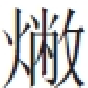
\includegraphics[width=4mm]{../images/00028}的胡说了。等我起来打不死你这小蹄子!''荳官见他要勾来,怎容他起来,便忙连身将他压倒。回头笑着央告蕊官等:``你们来帮着我拧他这诌嘴。''两个人滚在草地下。众人拍手笑说:``了不得了,那是一洼子水,可惜污了他的新裙子了。''荳官回头看了一看,果见旁边有一汪积雨,香菱的半扇裙子都污湿了,自己不好意思,忙夺了手跑了。众人笑个不住,怕香菱拿他们出气,也都哄笑一散。

香菱起身低头一瞧,那裙上犹滴滴点点流下绿水来。正恨骂不绝,可巧宝玉见他们斗草,也寻了些花草来凑戏,忽见众人跑了,只剩了香菱一个低头弄裙,因问:``怎么散了?''香菱便说:``我有一枝夫妻蕙,他们不知道,反说我诌,因此闹起来,把我的新裙子也脏了。''宝玉笑道:``你有夫妻蕙,我这里倒有一枝并蒂菱。''口内说,手内却真个拈着一枝并蒂菱花,又拈了那枝夫妻蕙在手内。香菱道:``什么夫妻不夫妻,并蒂不并蒂,你瞧瞧这裙子。''宝玉方低头一瞧,便``嗳呀''了一声,说:``怎么就拖在泥里了?可惜这石榴红绫最不经染。''香菱道:``这是前儿琴姑娘带了来的。姑娘做了一条,我做了一条,今儿才上身。''宝玉跌脚叹道:``若你们家,一日遭踏这一百件也不值什么。只是头一件既系琴姑娘带来的,你和宝姐姐每人才一件,他的尚好,你的先脏了,岂不辜负他的心。二则姨妈老人家嘴碎,饶这么样,我还听见常说你们不知过日子,只会遭踏东西,不知惜福呢。这叫姨妈看见了,又说一个不清。''香菱听了这话,却碰在心坎儿上,反倒喜欢起来了,因笑道:``就是这话了。我虽有几条新裙子,都不和这一样,若有一样的,赶着换了,也就好了。过后再说。''宝玉道:``你快休动,只站着方好,不然连小衣儿膝裤鞋面都要拖脏。我有个主意:袭人上月做了一条和这个一模一样的,他因有孝,如今也不穿。竟送了你换下这个来,如何?''香菱笑着摇头说:``不好。他们倘或听见了倒不好。''宝玉道:``这怕什么。等他们孝满了,他爱什么难道不许你送他别的不成。你若这样,还是你素日为人了!况且不是瞒人的事,只管告诉宝姐姐也可,只不过怕姨妈老人家生气罢了。''香菱想了一想有理,便点头笑道:``就是这样罢了,别辜负了你的心。我等着你,千万叫他亲自送来才好。''

宝玉听了,喜欢非常,答应了忙忙的回来,一壁里低头心下暗算:``可惜这么一个人,没父母,连自己本姓都忘了,被人拐出来,偏又卖与了这个霸王。''因又想起上日平儿也是意外想不到的,今日更是意外之意外的事了。一壁胡思乱想,{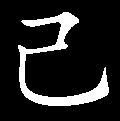
\includegraphics[width=3mm]{../Images/00003}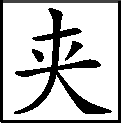
\includegraphics[width=3mm]{../Images/00012}\footnotesize \kaishu 又下此四字。}来至房中,拉了袭人,细细告诉了他原故。香菱之为人,无人不怜爱的。袭人又本是个手中撒漫的,况与香菱素相交好,一闻此信,忙就开箱取了出来折好,随了宝玉来寻着香菱,他还站在那里等呢。袭人笑道:``我说你太淘气了,足的淘出个故事来才罢。''香菱红了脸,笑说:``多谢姐姐了,谁知那起促狭鬼使黑心。''说着,接了裙子,展开一看,果然同自己的一样。又命宝玉背过脸去,自己叉手向内解下来,将这条系上。袭人道:``把这脏了的交与我拿回去,收拾了再给你送来。你若拿回去,看见了也是要问的。''香菱道:``好姐姐,你拿去不拘给那个妹妹罢。我有了这个,不要他了。''袭人道:``你倒大方的好。''香菱忙又万福道谢,袭人拿了脏裙便走。

香菱见宝玉蹲在地下,将方才的夫妻蕙与并蒂菱用树枝儿抠了一个坑,先抓些落花来铺垫了,将这菱蕙安放好,又将些落花来掩了,方撮土掩埋平服。香菱拉他的手,笑道:``这又叫做什么?怪道人人说你惯会鬼鬼祟祟使人肉麻的事。你瞧瞧,你这手弄的泥乌苔滑的,还不快洗去。''宝玉笑着,方起身走了去洗手,香菱也自走开。二人已走远了数步,香菱复转身回来叫住宝玉。宝玉不知有何话,扎着两只泥手,笑嘻嘻的转来问:``什么?''香菱只顾笑。因那边他的小丫头臻儿走来说:``二姑娘等你说话呢。''香菱方向宝玉道:``裙子的事可别向你哥哥说才好。''说毕,即转身走了。宝玉笑道:``可不我疯了,往虎口里探头儿去呢。''说着,也回去洗手去了。不知端详,且听下回分解。

{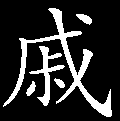
\includegraphics[width=3mm]{../Images/00005}总评:写寻闹是贾母不在家景况,写设筵亦是贾母不在家景况。如此说来,如彼说来,真有笔歌墨舞之乐。}

{看湘云醉卧青石,满身花影,宛若百十名姝,抱云笙月鼓而簇拥太真者。}

%{\href{../Text/part0066_split_000.html\#navto_1_a}{①}``鸳鸯赢了尤氏'',原缺,据戚本补。按此处鸳鸯与袭人均是赢家,但后文写鸳鸯、袭人说俗语完令,则似乎两人又是输家了。原文如此,存疑待考。}
